\documentclass{article}
\usepackage[x11names, svgnames, rgb]{xcolor}
\usepackage[utf8]{inputenc}
\usepackage{tikz}
\usetikzlibrary{snakes,arrows,shapes}
\usepackage{amsmath}
\definecolor{lightcoral}{RGB}{240,128,128}
\definecolor{lightgreen}{RGB}{144,238,144}
%
%

%

%

\begin{document}
\pagestyle{empty}
%
%
%

\enlargethispage{100cm}
% Start of code
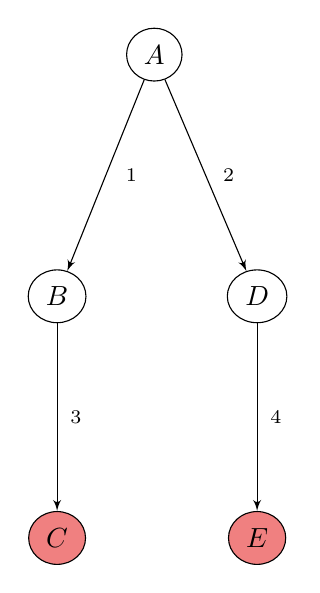
\begin{tikzpicture}[>=latex',line join=bevel,]
%%
\node (A) at (62.0bp,192.0bp) [draw,ellipse] {$A$};
  \node (B) at (27.0bp,105.0bp) [draw,ellipse] {$B$};
  \node (D) at (99.0bp,105.0bp) [draw,ellipse] {$D$};
  \node (C) at (27.0bp,18.0bp) [draw,fill=lightcoral,ellipse] {$C$};
  \node (E) at (99.0bp,18.0bp) [draw,fill=lightcoral,ellipse] {$E$};
  \draw [->] (A) ..controls (50.031bp,162.25bp) and (43.441bp,145.87bp)  .. (B);
  \definecolor{strokecol}{rgb}{0.0,0.0,0.0};
  \pgfsetstrokecolor{strokecol}
  \draw (54.0bp,148.5bp) node {$_1$};
  \draw [->] (A) ..controls (74.653bp,162.25bp) and (81.62bp,145.87bp)  .. (D);
  \draw (89.0bp,148.5bp) node {$_2$};
  \draw [->] (B) ..controls (27.0bp,75.192bp) and (27.0bp,59.561bp)  .. (C);
  \draw (34.0bp,61.5bp) node {$_3$};
  \draw [->] (D) ..controls (99.0bp,75.192bp) and (99.0bp,59.561bp)  .. (E);
  \draw (106.0bp,61.5bp) node {$_4$};
%
\end{tikzpicture}
% End of code

%
\end{document}
%



